\chapter{Interação Gestual e Hiperinstrumentos}
\label{cap:interacao_gestual_e_hiperinstrumentos}

Neste capítulo, a fundamentação teórica que orientou o projeto (\textit{design}) e os objetivos do Aerochord é aprofundada. Inicialmente, na seção \ref{sec:iteracao_multimodal}, o campo da Interação Humano-Computador (IHC) é explorado, destacando-se o paradigma da interação gestual como uma modalidade de controle expressiva e natural, capaz de resgatar a corporeidade e a nuance da execução musical (\textit{performance}). Em seguida, na seção \ref{sec:dispositivos_e_ferramentas_deteccao_gestos}, são examinadas as principais ferramentas e tecnologias de detecção de gestos, com ênfase em abordagens de visão computacional que fundamentaram a solução técnica adotada no projeto. Por fim, na seção \ref{sec:hiperinstrumentos_musicais} apresenta-se e discute-se o conceito de hiperinstrumento, arcabouço conceitual (\textit{framework}) que define a natureza do instrumento materializado pelo Aerochord: um sistema musical gestual de alta expressividade, acessível e extensível. Assim, é apresentado um panorama organizado das bases teóricas e tecnológicas que sustentam o desenvolvimento do projeto, mostrando como os temas abordados — a interação gestual na IHC, as técnicas de detecção e o conceito de hiperinstrumento — se relacionam para fundamentar a arquitetura da solução.

\section{Interação Multimodal e Gestual}
\label{sec:iteracao_multimodal}

A área de Interação Humano-Computador (IHC) tem como objetivo superar as restrições impostas por interfaces convencionais, como teclado e \textit{mouse} (dispositivo apontador), ao buscar meios de interação mais naturais, intuitivos e centrados nas capacidades humanas. À medida que sistemas computacionais se integram de forma crescente ao cotidiano, surge a demanda por interfaces que reflitam a fluidez e a riqueza da comunicação interpessoal, reduzindo a distância entre a intenção do usuário e a resposta do sistema. Esse contexto justificou a investigação de modalidades gestuais no projeto Aerochord, por se tratar de uma abordagem que aproxima a interação digital dos modos como as pessoas se comunicam entre si \cite{preece2023interaction}.

\subsection{O Paradigma da Interação Multimodal}
\label{subsec:paradigma_iteracao_multimodal}

Sistemas multimodais são aqueles capazes de processar, de maneira coordenada, múltiplas modalidades de entrada, como fala, gestos, olhar e toque, de modo que cada canal contribua para uma interpretação mais precisa da intenção do usuário. Por meio de fusão de sinais e integração temporal e semântica, esses sistemas combinam fluxos sensoriais distintos para aumentar a robustez e a adaptabilidade da interface. Isso permite que falhas ou ambiguidades em um modo sejam compensadas por outro. 

Essa coordenação entre canais também oferece flexibilidade, pois o usuário pode escolher a modalidade mais conveniente conforme o contexto e suas preferências. Além disso, promove maior naturalidade ao refletir padrões típicos da comunicação entre pessoas \cite{oviatt2018multimodal2, oviatt2019multimodal3}. Interfaces multimodais também conseguem se adaptar dinamicamente a mudanças ambientais, alternando ou combinando modos de entrada para manter a eficácia da interação. Esses fatores justificam o estudo aprofundado de modalidades específicas, como a gestual, dentro de um quadro multimodal mais amplo.

A multimodalidade confere vantagens centrais em termos de usabilidade: flexibilidade para o usuário selecionar o canal mais adequado, robustez ao mitigar falhas em uma modalidade por meio de outra, e maior naturalidade ao espelhar padrões comunicativos humanos. Tais benefícios reforçam a importância do estudo de interfaces gestuais, mesmo em projetos que foquem primariamente nessa modalidade, pois elas se inserem num ecossistema de interação que visa experiências mais ricas e resilientes \cite{oviatt2019multimodal3}.

\subsection{A Expressividade da Interação Gestual na Música}
\label{subsec:expressividade_iteracao_gestual}

A interação gestual \textit{mid-air} (gestos realizados no ar) refere-se a movimentos livres de mãos e braços no espaço, sem contato físico com superfícies, proporcionando potencial expressivo elevado, mas impondo desafios ergonômicos, perceptuais e técnicos. Entre esses desafios estão a fadiga muscular decorrente de gestos prolongados, a ausência de retorno (\textit{feedback}) tátil natural, as variações de iluminação e cenário que afetam a detecção, e a necessidade de latência muito baixa para manter a sensação de controle imediato. Além disso, torna-se necessário incorporar \textit{feedback} audiovisual ou háptico (relativo ao tato) artificial para confirmar o reconhecimento dos gestos \cite{aigner2012understanding}. Esses aspectos exigem projetos cuidadosos de detecção, filtragem de ruído e mecanismos de confirmação, de modo a preservar a fluidez e a confiança do usuário na interface gestual.

Contudo, habilitar controle por gestos não é suficiente; é imprescindível que o repertório gestual seja intuitivo e fácil de aprender. Metodologias formais de elicitação de gestos para interação \textit{mid-air} são aplicadas com o objetivo de identificar movimentos que os usuários associam espontaneamente a determinadas ações. Esse raciocínio orientou o mapeamento no Aerochord, garantindo que os gestos implementados coincidissem com expectativas naturais e se mantivessem ergonômicos, evitando movimentos excessivamente amplos ou complexos que pudessem comprometer a experiência \cite{vogiatzidakis2018gesture}.

No contexto musical, gestos e som estão intrinsecamente conectados. Em instrumentos tradicionais, a execução sonora já se baseia em atos gestuais refinados, nos quais movimentos sutis determinam nuances de timbre, dinâmica e articulação. Controlar sistemas digitais por meio de gestos busca resgatar essa corporeidade, permitindo manipulações contínuas e multidimensionais de vários parâmetros sonoros (posição, velocidade, aceleração, trajetória e intensidade) que interfaces convencionais dificilmente capturam com fidelidade. Estudos na área de controle gestual musical mostram que a riqueza e a precisão dos dados capturados influenciam diretamente a expressividade do intérprete, reforçando que a modalidade gestual é especialmente poderosa e natural para expressão sonora \cite{wanderley2001gestural, cadoz2000gesture}.

Em síntese, os princípios de IHC e multimodalidade discutidos nesta seção reforçam a importância de interfaces mais humanas. Dentre essas, a interação gestual \textit{mid-air} se destaca como particularmente relevante para a música digital, pois tem o potencial de recuperar nuances e a corporeidade típicas da performance tradicional. É com base nessa fundamentação teórica que o Aerochord propôs e implementou um sistema de controle gestual via visão computacional, criando uma experiência musical intuitiva e acessível. Na seção seguinte, são detalhadas as tecnologias de detecção de gestos que viabilizam essa interação.

\section{Dispositivos e Ferramentas para Detecção de Gestos}
\label{sec:dispositivos_e_ferramentas_deteccao_gestos}

Capturar e interpretar gestos humanos de forma precisa constitui um dos principais desafios na IHC, pois envolve traduzir movimentos físicos contínuos e tridimensionais em dados digitais compreensíveis por um sistema computacional. Conforme discutido por Preece, Sharp e Rogers (\citeyear{preece2023interaction}), a complexidade dessa tarefa decorre da variabilidade natural dos usuários, das condições ambientais e da necessidade de resposta em tempo real para aplicações interativas. Para “sensoriar” gestos, diversas tecnologias foram desenvolvidas, cada qual com benefícios e limitações próprias no que tange à precisão, ao custo e à dependência de equipamento físico (\textit{hardware}) específico. É fundamental, portanto, compreender essas categorias de solução a fim de situar a escolha para o projeto Aerochord dentro de um contexto de acessibilidade e robustez.

Uma das abordagens pioneiras e mais influentes baseia-se em câmeras de profundidade, que utiliza luz infravermelha para medir a distância de cada ponto da cena até o sensor, permitindo segmentar o usuário do fundo e estimar a posição tridimensional das articulações. O Microsoft Kinect (Figura \ref{kinect}) tornou-se referência ao empregar essa técnica para rastreamento esquelético em tempo real. O método proposto por Shotton et al., baseado em florestas aleatórias (\textit{random forests}) treinadas com grandes volumes de dados sintéticos, possibilita classificar cada pixel da imagem de profundidade em partes do corpo, gerando estimativas rápidas e precisas das juntas corporais \cite{shotton2011real}. Apesar de sua eficácia, essa solução demanda \textit{hardware} específico (sensor de profundidade dedicado) e, embora tenha impulsionado pesquisas em IHC, limita-se em termos de acessibilidade e portabilidade para projetos que buscam operar com dispositivos amplamente disponíveis.

\begin{figure}[htbp!]
	\caption{Dispositivo Microsoft Kinect, modelo do console Xbox 360}
	\centering 
	\label{kinect}
	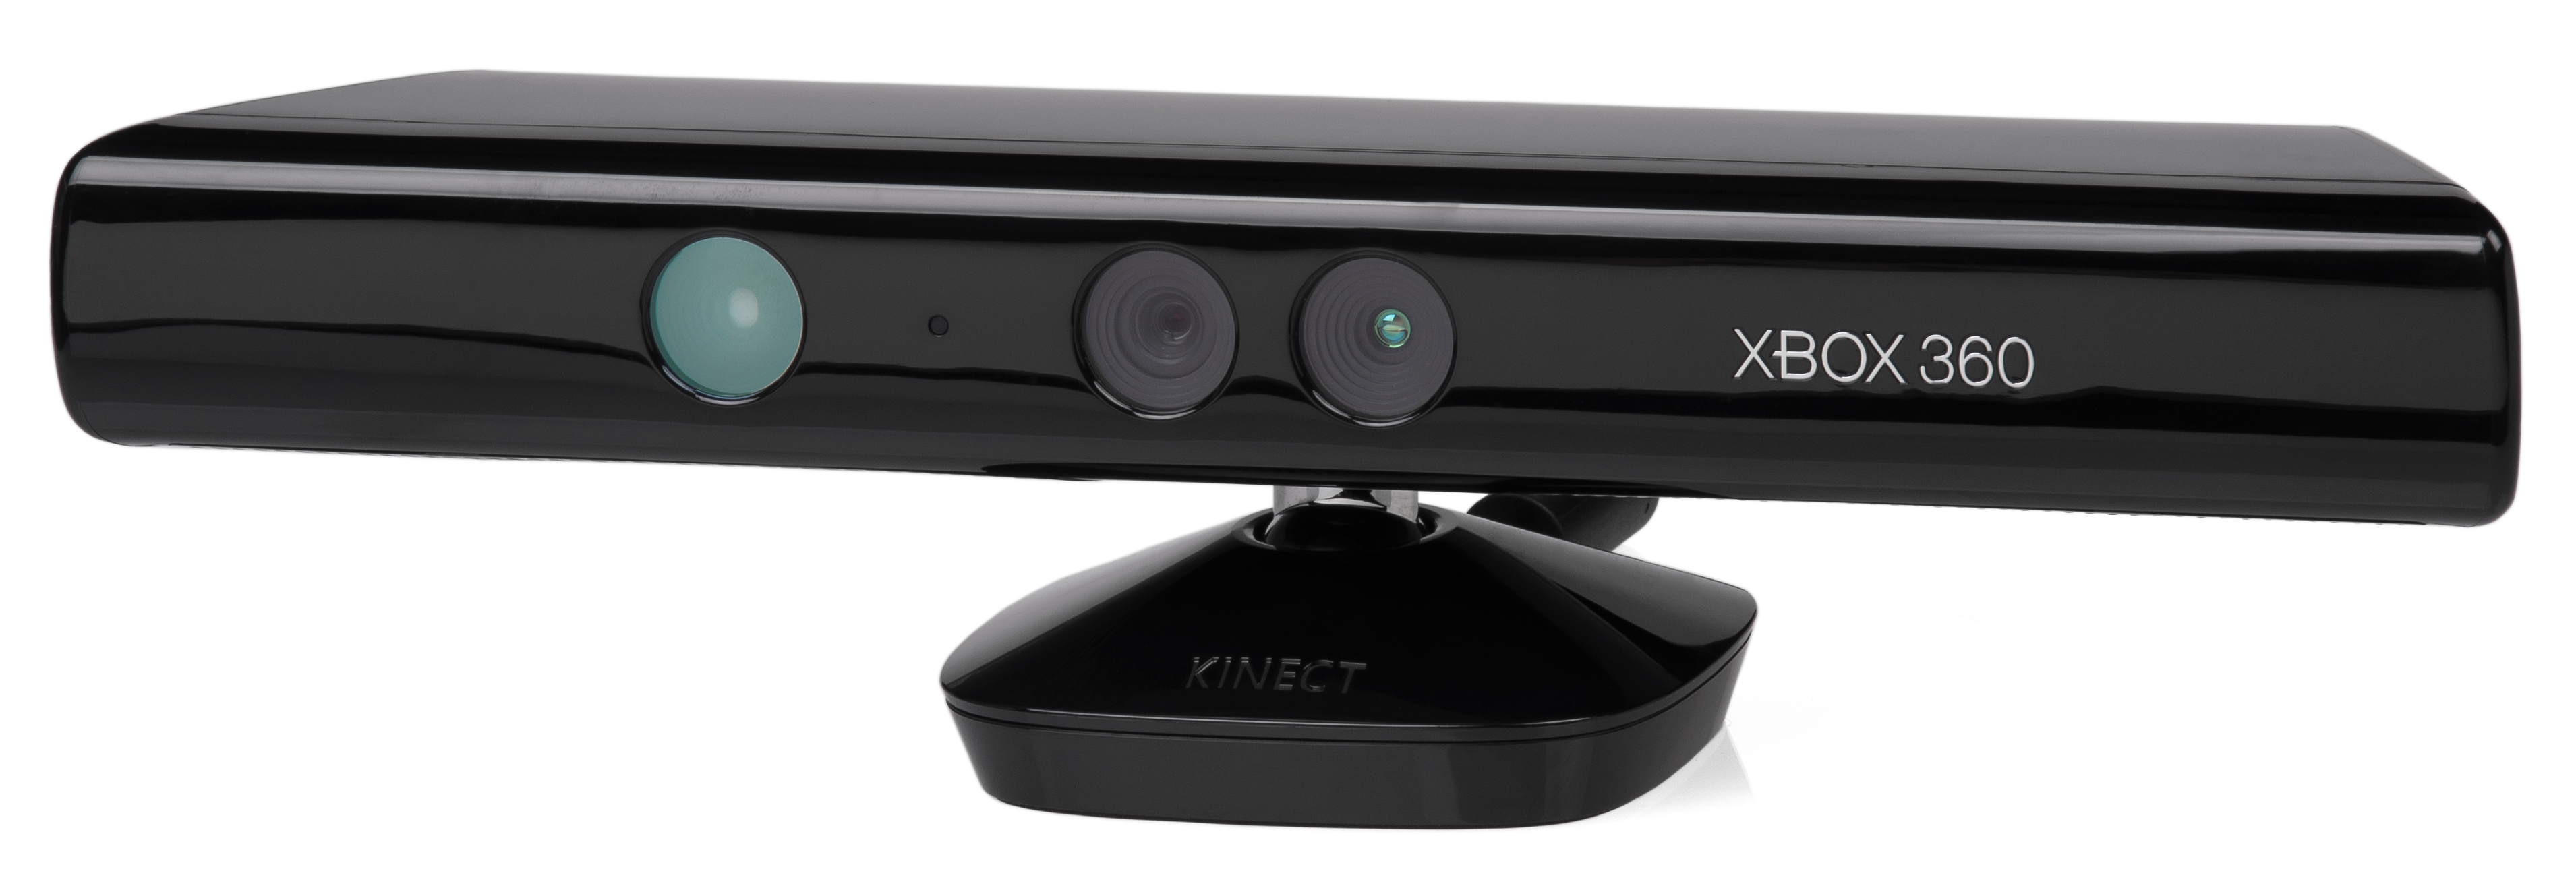
\includegraphics[width=0.4\linewidth]{imagens/kinect.png}
    \fonte{Disponível em: <https://pt.wikipedia.org/wiki/Kinect>. Acesso em 23 jun. 2025}
\end{figure}

Outra categoria relevante envolve controladores dedicados ao rastreamento manual, como o Leap Motion Controller (Figura \ref{leapmotion}). Zhang et al. (\citeyear{zhang2019gestureteleop}) demonstram sua aplicação em sistemas de teleoperação baseados em gestos, evidenciando a capacidade do dispositivo em detectar movimentos das mãos e dedos com alta precisão e baixa latência para aplicações em controle de robôs. Embora esse tipo de dispositivo ofereça alto desempenho para detecção de gestos precisos, ele também implica custo adicional de \textit{hardware} especializado, além de restringir o espaço de interação ao volume monitorado pelo sensor, o que contrasta com a meta do Aerochord de empregar soluções de baixo custo e maior flexibilidade.

\begin{figure}[htbp!]
	\caption{Controlador Leap Motion em uso para rastreamento de movimentos das mãos}
	\centering 
	\label{leapmotion}
	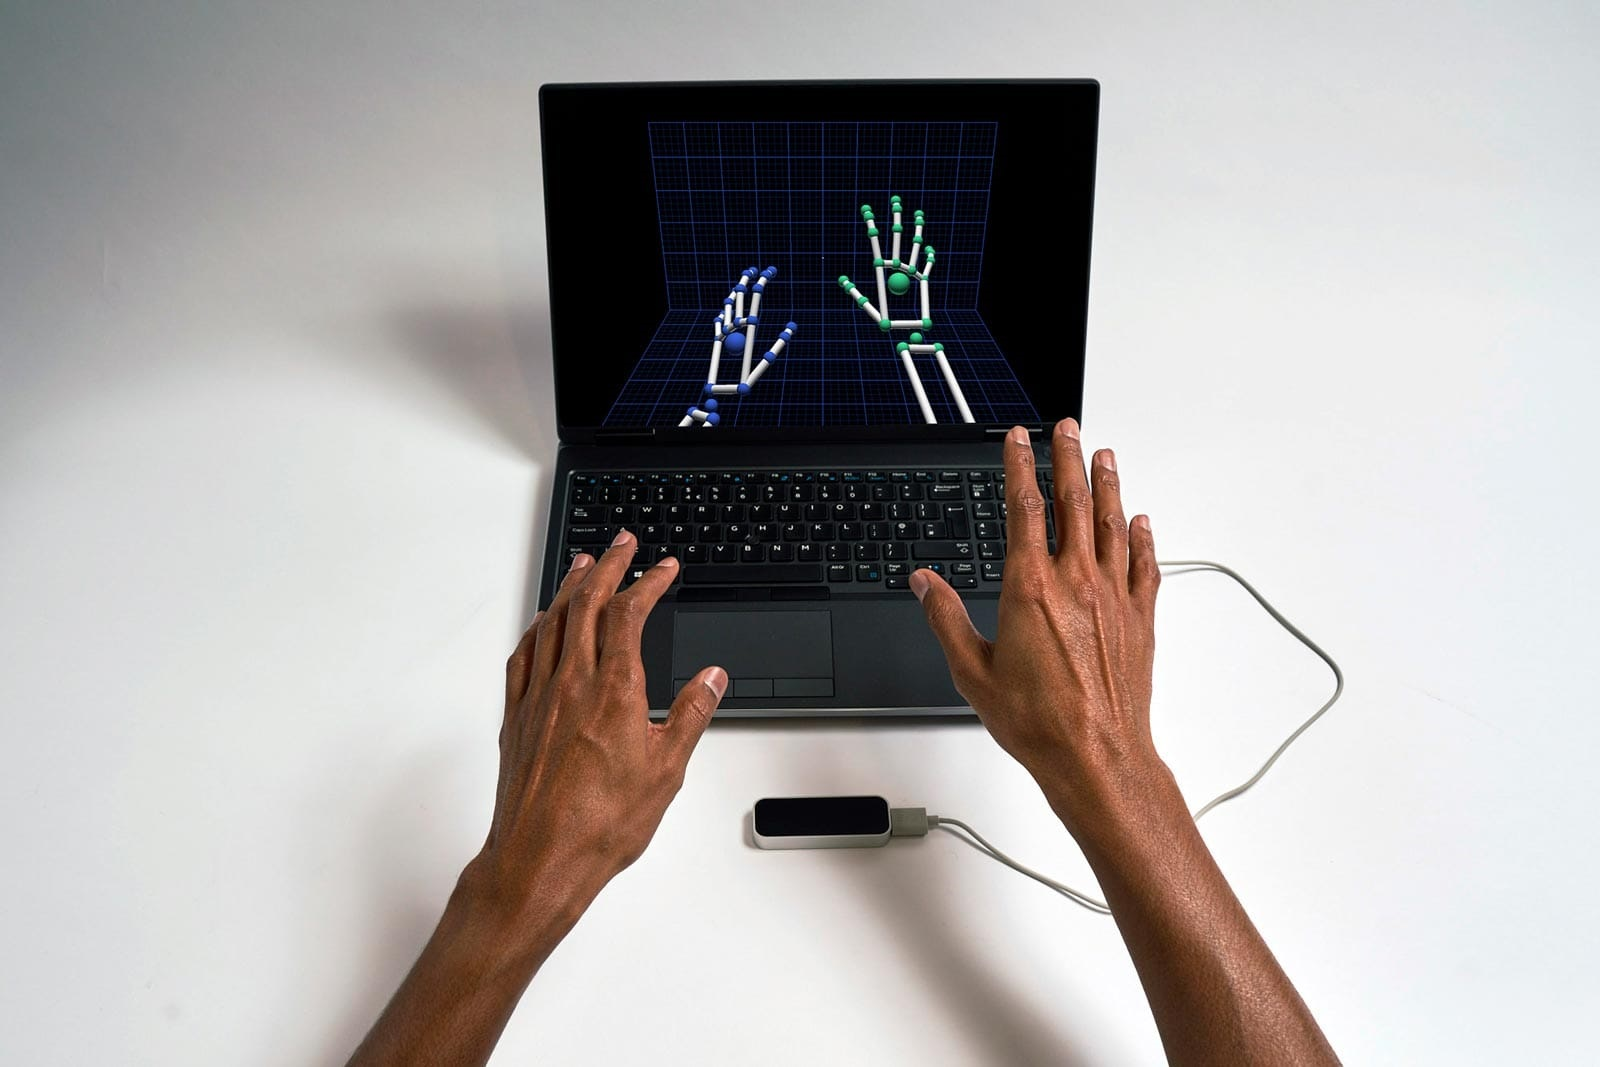
\includegraphics[width=0.55\linewidth]{imagens/LeapMotion.png}
    \fonte{Disponível em: <https://documentation.ls-group.fr/interact/LeapMotion/>. Acesso em 23 jun. 2025}
\end{figure}

No campo de sensores vestíveis (\textit{wearables}), destacam-se as chamadas luvas de dados (\textit{data gloves}) (Figura \ref{cyberglove}), que integram sensores de flexão e Unidades de Medição Inercial (IMUs) para medir diretamente os movimentos das mãos. A revisão feita por Dipietro et al. (\citeyear{dipietro2008survey}), aponta como pontos positivos a alta fidelidade na captura de ângulos articulares e ausência de problemas de oclusão visual, mas também ressalta desvantagens como o custo elevado, necessidade de calibração constante e caráter invasivo da interface, que pode prejudicar a naturalidade da interação. Essa categoria, embora tecnicamente robusta, também se afasta do objetivo do Aerochord de oferecer expressão musical sem impor acessórios ao usuário.

\begin{figure}[htbp!]
	\centering
	\caption{Luva de dados CyberGlove III projetada pela CyberGlove Systems}
	\label{cyberglove}
    \begin{subfigure}{0.36\textwidth}
		\centering
		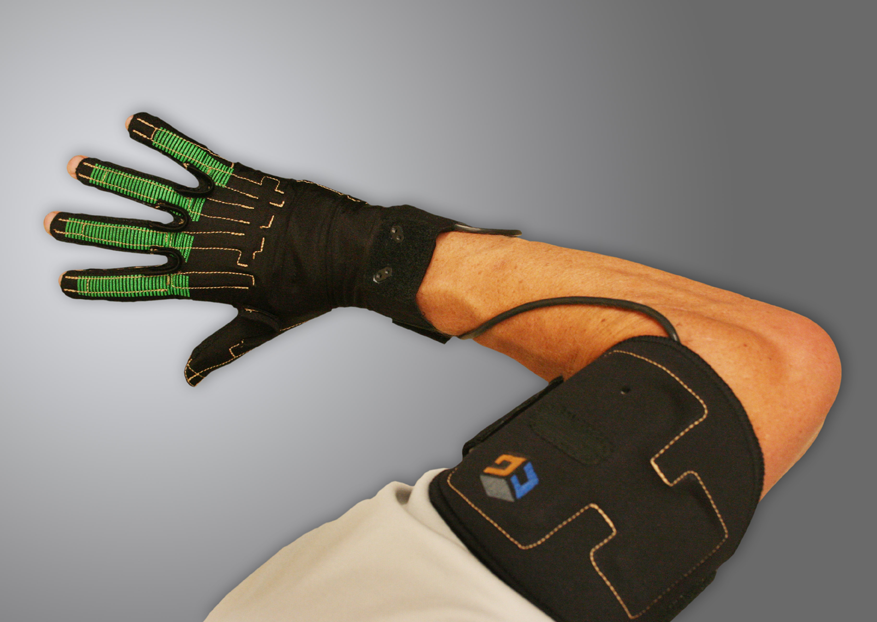
\includegraphics[width = \textwidth]{imagens/CyberGloveIII.png}
		\caption{Sensor vestível CyberGlove III}
		\label{fig:cyberglove_sensor}
	\end{subfigure}
    \begin{subfigure}{0.50\textwidth}
		\centering
		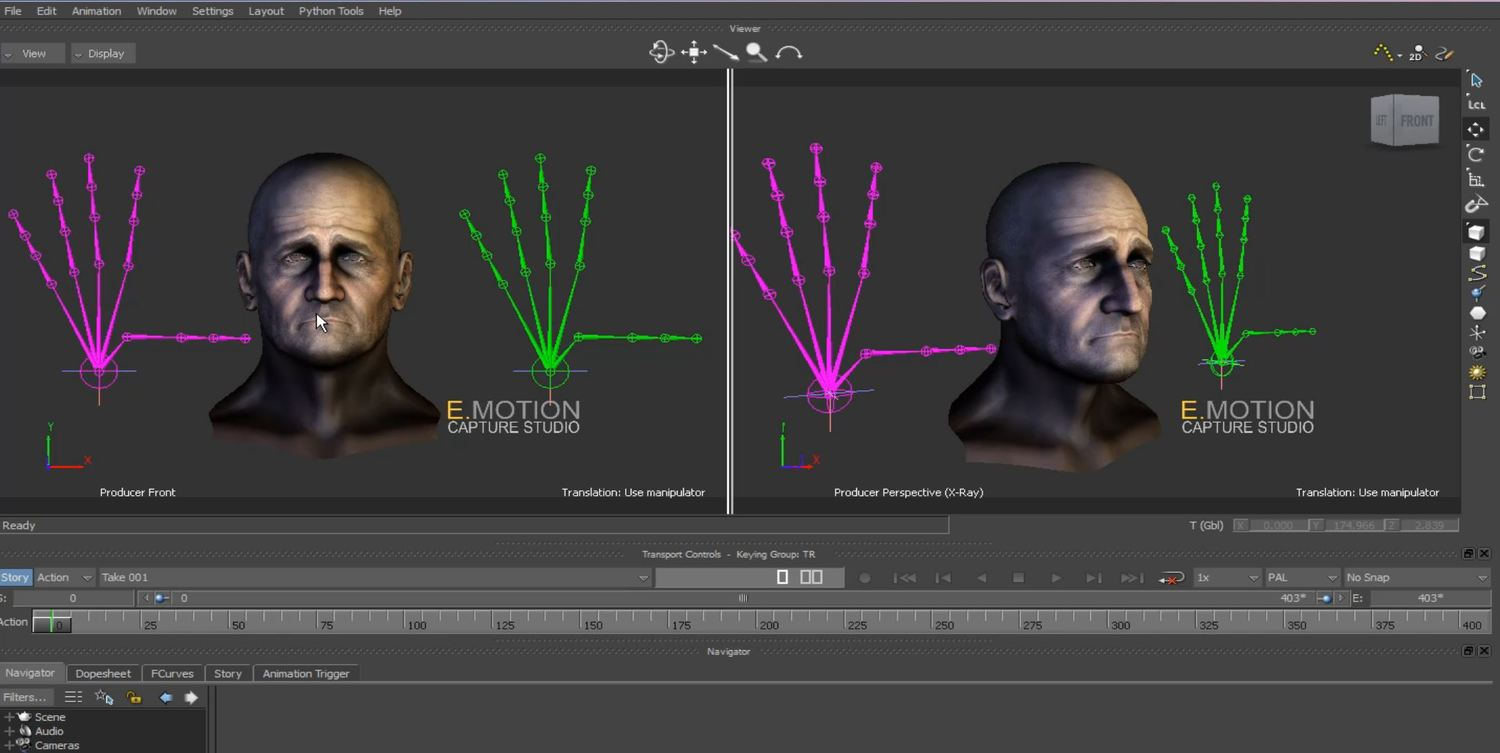
\includegraphics[width = \textwidth]{imagens/software_cyber_glove.jpg}
		\caption{\textit{Software} interpretando os comandos enviados pela CyberGlove III}
		\label{fig:cyberglove_software}
	\end{subfigure}
	\fonte{Disponível em: <https://www.cyberglovesystems.com/cyberglove-iii/>. Acesso em 23 jun. 2025}
\end{figure}

Adicionalmente, avanços em inteligência artificial e visão computacional têm viabilizado o rastreamento de gestos utilizando apenas câmeras RGB comuns, como \textit{webcams}. Rautaray e Agrawal (\citeyear{rautaray2012vision}) apresentam uma revisão de técnicas de reconhecimento de gestos baseadas em visão, destacando fases de detecção, rastreamento e reconhecimento que exploram desde segmentação de pele até modelos de aprendizado profundo (\textit{deep learning}) para extrair características das mãos em imagens bidimensionais (2D). Essa abordagem mostra-se promissora para aplicações acessíveis, uma vez que aproveita \textit{hardware} amplamente disponível e avanços em algoritmos que toleram variações de iluminação e cenários diversos, conectando-se diretamente ao objetivo do Aerochord de democratizar o controle gestual musical.

Entre as ferramentas de visão computacional para detecção de gestos, destaca-se o MediaPipe, \textit{framework} de código aberto (\textit{open source}) desenvolvido pelo Google, que oferece esteiras de processamento (\textit{pipelines}) pré-configuradas de aprendizado de máquina (\textit{machine learning}) para rastreamento de mãos e poses corporais em tempo real. Conforme descrito por Lugaresi et al. (\citeyear{lugaresi2019mediapipe}), o MediaPipe permite construir grafos de processamento de vídeo que interpretam o fluxo capturado pela \textit{webcam} e entregam, em tempo real, coordenadas tridimensionais (3D) estimadas dos pontos-chave das mãos, com desempenho otimizado para várias plataformas. A documentação oficial do projeto também fornece instruções detalhadas para a personalização e integração desses módulos em aplicações específicas \cite{mediapipeWebsite}. Por combinar alta precisão, baixa latência e depender apenas de \textit{hardware} onipresente, o MediaPipe consolidou-se como a base tecnológica do Aerochord, atendendo perfeitamente aos requisitos de expressividade musical e acessibilidade pretendidos.

\section{Hiperinstrumentos Musicais}
\label{sec:hiperinstrumentos_musicais}

A evolução dos instrumentos musicais na era digital pode ser entendida como uma extensão da longa história de refinamento das interfaces físicas entre o artista e o som, agora estendendo-se para além das restrições mecânicas e acústicas tradicionais em direção a sistemas computadorizados que ampliam as possibilidades expressivas. Conforme argumentado por Wanderley (\citeyear{wanderley2001gestural}), instrumentos digitais não sofrem as mesmas limitações físicas de tubos, cordas ou membranas, permitindo uma diversidade enorme de métodos de produção sonora. No entanto, para que esses sistemas ofereçam controle refinado comparável ao das famílias acústicas clássicas, estratégias de projeto cuidadosas de mapeamento e de interface devem ser definidas.

\subsection{Definição e Características}
\label{sec:definicao_e_caracteristicas}

Em 1986, Tod Machover fundou o grupo Hyperinstruments no \textit{MIT Media Lab}, formalizando o conceito de hiperinstrumento como uma extensão tecnológica da prática musical. Segundo o autor,  esse tipo de sistema é composto por três elementos fundamentais: (1) uma interface sensorial para o \textit{performer}\footnote{Pessoa que executa um instrumento, seja ele tradicional ou digital (\textit{performer}).}, capaz de capturar gestos, toques ou outras ações; (2) um módulo de processamento, que analisa e interpreta os dados de performance em tempo real; e (3) um sistema de geração ou modulação sonora, que pode envolver síntese digital, modelagem física ou controle de sintetizadores via protocolos como MIDI \cite{Machover1992}. No contexto do Aerochord, esses três componentes alinham-se da seguinte forma: a interface é o corpo do usuário capturado por visão computacional; o módulo de processamento é o \textit{software} em C++ que extrai pontos-chave e gestos (via MediaPipe); e o gerador sonoro pode ser qualquer sintetizador compatível com MIDI 2.0, acionado via \textit{Universal MIDI Packets}.

Machover (\citeyear{Machover1992}) enfatiza também a filosofia de aumentação em vez de mera substituição: não se trata apenas de criar timbres novos, mas de capturar nuances da performance humana (velocidade, aceleração, pressão, gestos sutis) que muitas vezes ficam fora do alcance de controles convencionais, e usar esses dados para controlar parâmetros sonoros de forma rica e multidimensional. Essa perspectiva de ampliar a expressividade natural do \textit{performer} reflete o objetivo de hiperinstrumentos de explorar dimensões de controle além do que um instrumento acústico isolado permitiria, usando o poder computacional para traduzir sutilezas gestuais em transformações sonoras complexas.

\subsection{Evolução e Exemplos Notáveis}
\label{sec:evolucao_e_exemplos_notaveis}

Historicamente, desvincular o gesto da produção sonora mecânica precede a era dos computadores. Instrumentos como o Theremin (Figura \ref{theremin}), criado em 1920, e o Ondes Martenot, desenvolvido em 1928, romperam com a necessidade de contato físico direto, permitindo o controle de altura e volume ou de timbre e efeito de modulação de frequência (\textit{vibrato}) por gestos. No caso do Theremin, a proximidade das mãos em relação às antenas determinava as frequências geradas, enquanto o Ondes Martenot combinava um teclado com um anel deslizante para manipulação contínua de som. Esses instrumentos pioneiros anteciparam, em termos conceituais, a performatividade expandida dos hiperinstrumentos computadorizados, ao sugerirem novas formas de mediação gestual e controle expressivo \cite{Manning1993}.

\begin{figure}[htbp!]
	\caption{Léon Theremin, criador do Theremin, demonstrando seu instrumento}
	\centering 
	\label{theremin}
	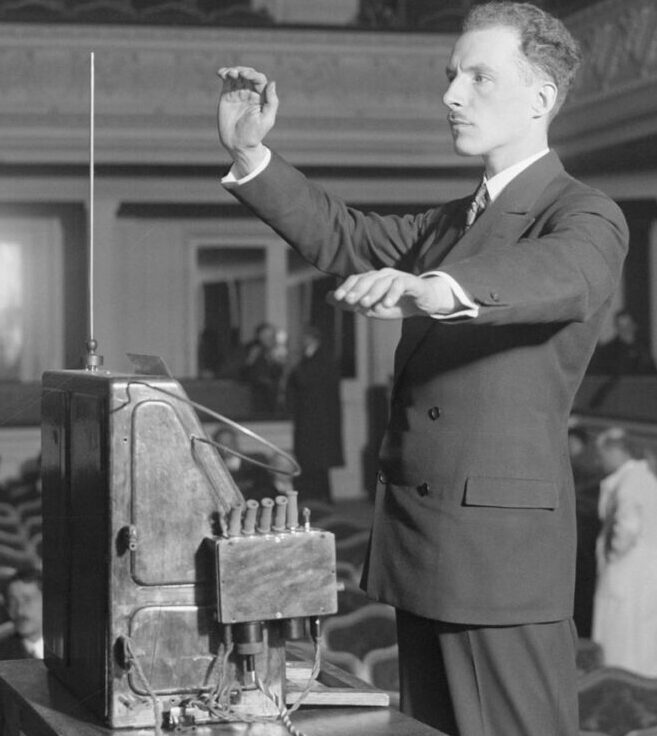
\includegraphics[width=0.24\linewidth]{imagens/theremin.jpg}
    \fonte{Disponível em: <https://en.wikipedia.org/wiki/Leon\_Theremin>. Acesso em 23 jun. 2025}
\end{figure}

A formalização do termo “hiperinstrumento” ocorreu em 1986, com o trabalho do grupo Hyperinstruments de Tod Machover. Um dos projetos mais emblemáticos desse período foi o Hypercello (Figura \ref{hypercello}), desenvolvido em 1991 por Machover em colaboração com o violoncelista Yo-Yo Ma, em que sensores no arco e no violoncelo capturavam parâmetros de performance (como pressão, velocidade e posição) e os convertiam em dados interpretados em tempo real para modificar aspectos do som, incluindo timbre, espacialização e efeitos. Esse modelo demonstra a aplicação prática dos três componentes definidos por Machover: o intérprete interage fisicamente (sensores no instrumento acústico), o computador processa os dados em tempo real, e o sistema sonoro responde de acordo com mapeamentos definidos, muitas vezes enriquecidos por algoritmos de síntese e processamento que ampliam o leque expressivo do instrumento original \cite{Machover1992}.

Em complemento aos projetos iniciais de Machover, Manning (\citeyear{Manning1993}) descreve também o \textit{Hyperbow Controller} (Figura \ref{hyperbow}), um arco de violino desenvolvido para uso com um violino elétrico. Esse dispositivo incorpora extensômetros (\textit{strain gauges}, sensores que medem deformação física) que medem as forças aplicadas no arco e acelerômetros que capturam variações de aceleração e inclinação durante o movimento. Essas informações gestuais são convertidas em múltiplos sinais de controle, que são processados em tempo real para modificar parâmetros como timbre, dinâmica e espacialização, sem comprometer a interação física familiar ao violinista. O \textit{Hyperbow} exemplifica a filosofia de aumentação em hiperinstrumentos, ampliando as possibilidades expressivas do gesto de arco tradicional ao traduzi-lo em comandos sonoros multidimensionais via síntese digital ou processamento computacional.

\begin{figure}[htbp!]
    \caption{Tod Machover e seu Hypercello}
    \centering 
    \label{hypercello}
    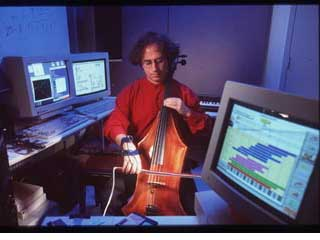
\includegraphics[width=0.75\linewidth]{imagens/hypercello.jpg}
    \fonte{Disponível em: <https://opera.media.mit.edu/projects/trilogy.html>. Acesso em 23 jun. 2025}
\end{figure}

\begin{figure}[htbp!]
    \caption{Hyperbow sendo utilizado em um violoncelo}
	\centering
    \label{hyperbow}
    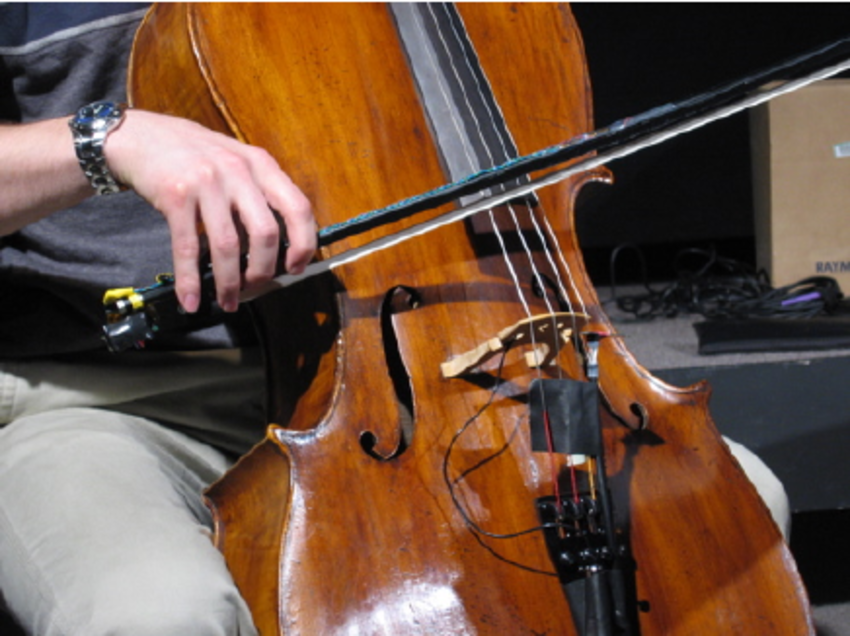
\includegraphics[width=0.6\linewidth]{imagens/hyperbow.png}
    \fonte{Disponível em: <https://www.researchgate.net/figure/Hyperbow-and-acoustic-acoustic-cello-C-Roberto-Aimi-Interestingly-although-the\_fig1\_221164872>. Acesso em 23 jun. 2025}
\end{figure}

Em tempos mais recentes, surgiram exemplos que empregam interfaces tangíveis e visuais para enriquecer a performance musical. Um exemplo é o Reactable (Figura \ref{reactable}), desenvolvido na \textit{Universitat Pompeu Fabra}, que consiste em uma superfície interativa sensível ao toque e à manipulação de objetos físicos, com visualização em tempo real para múltiplos usuários colaborarem musicalmente. Essa plataforma une o gesto manual direto a \textit{feedback} audiovisual, configurando uma forma contemporânea de hiperinstrumento que amplia a expressividade e a interação social em performance ao vivo \cite{weinerzl2017musical21}. Embora existam também controladores gestuais baseados em \textit{hardware} dedicado, a ênfase recente em visão computacional e sensores amplamente disponíveis reflete a busca por acessibilidade, alinhando-se diretamente ao projeto Aerochord, que visa empregar câmeras comuns para capturar gestos e oferecer controle musical sensível sem exigir dispositivos especializados.

\begin{figure}[htbp!]
    \caption{Reactable}
	\centering
    \label{reactable}
    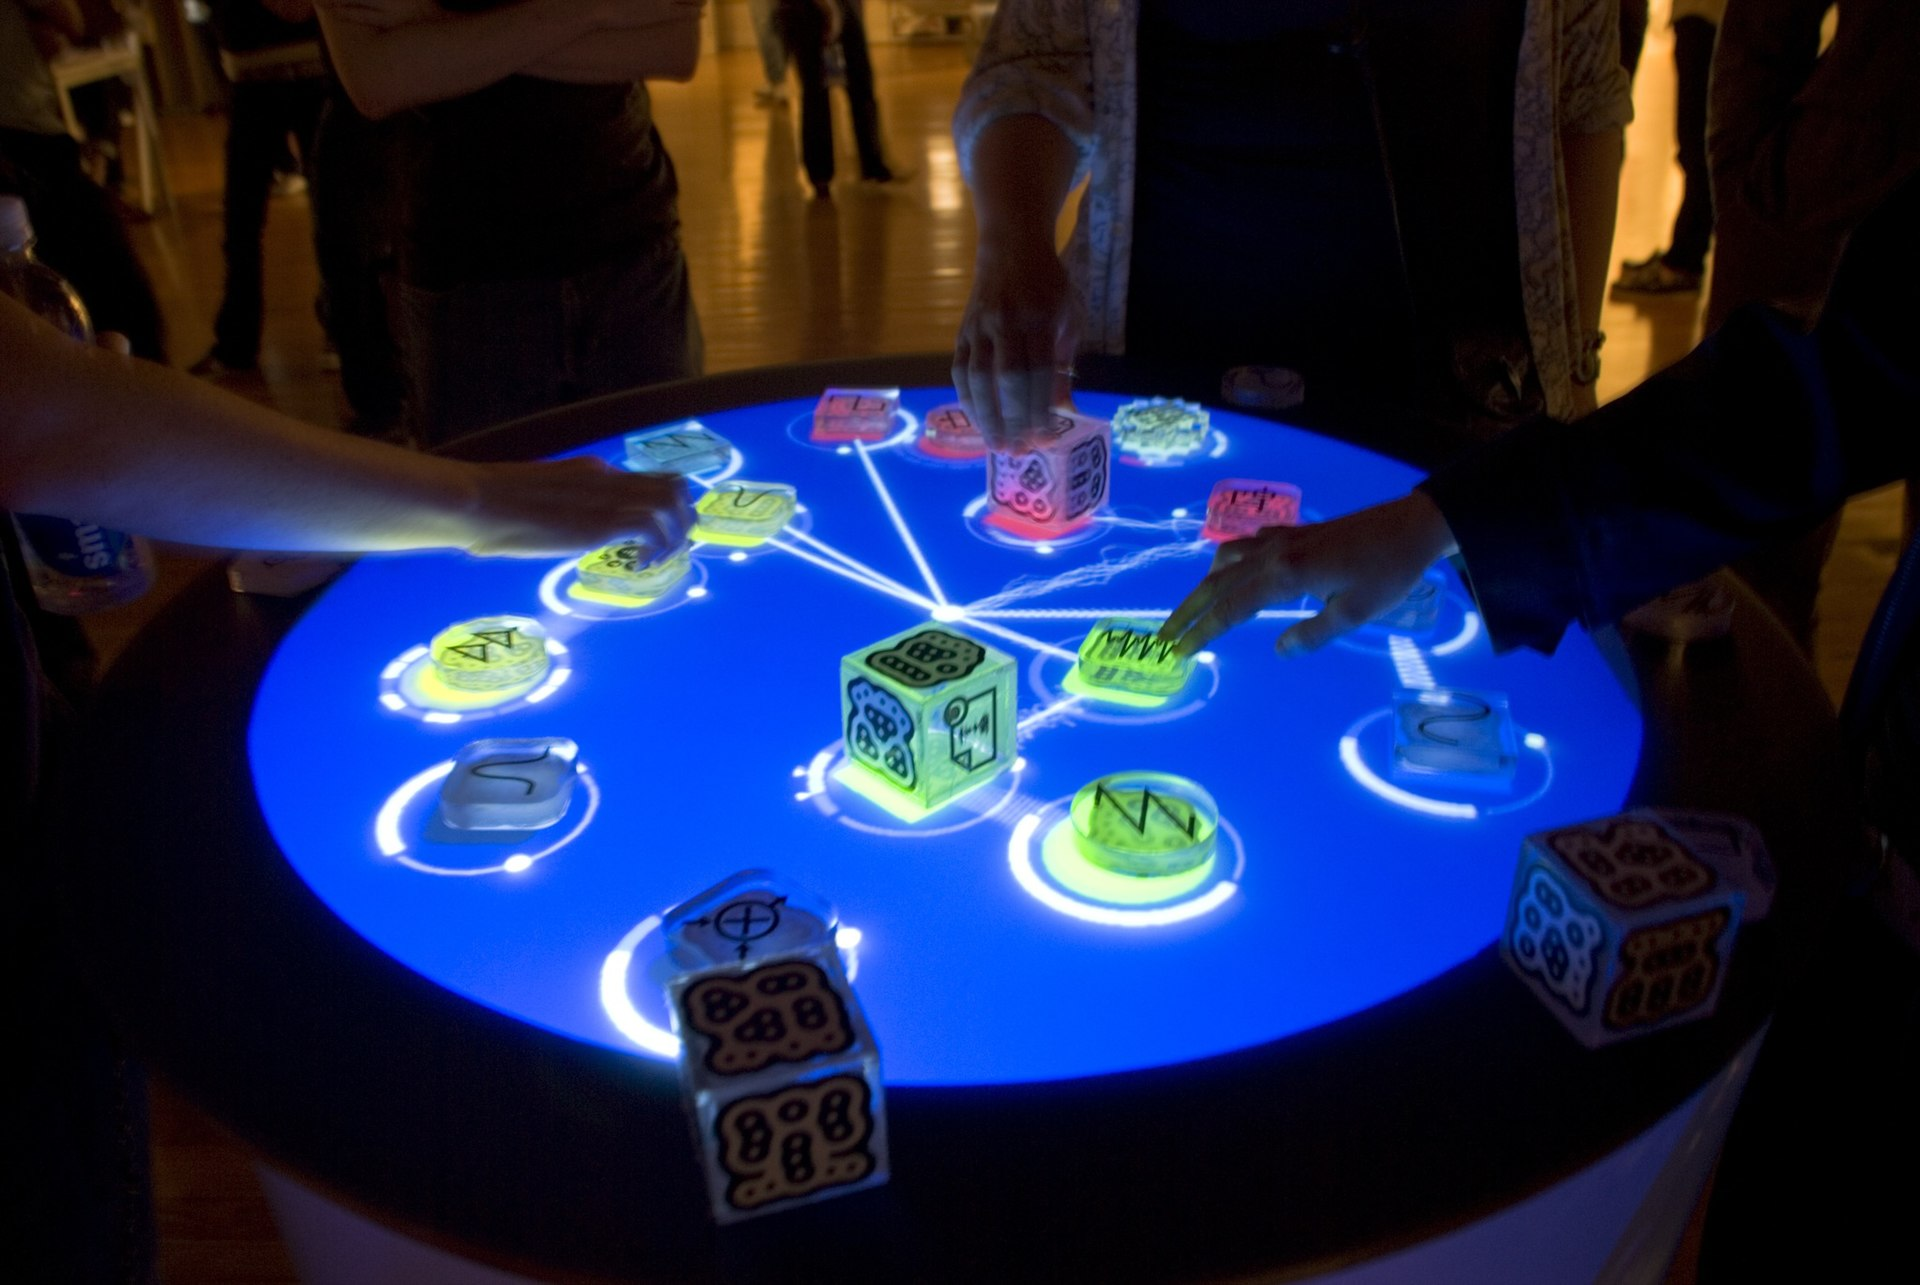
\includegraphics[width=0.5\linewidth]{imagens/reactable.jpg}
    \fonte{Disponível em: <https://en.wikipedia.org/wiki/Reactable>. Acesso em 23 jun. 2025}
\end{figure}

\subsection{Hiperinstrumentos e Interação Gestual}
\label{sec:hiperinstrumentos_e_interacao_gestual}

A interação gestual ocupa papel central no \textit{design} de hiperinstrumentos, pois permite capturar a expressividade natural do corpo do \textit{performer} de modo contínuo e multidimensional. Conforme argumenta Wanderley (\citeyear{wanderley2001gestural}), o gesto musical, especialmente em instrumentos acústicos, já é uma forma de controle multiparamétrico, envolvendo aspectos como sincronização rítmica (\textit{timing}), articulação e dinâmica. Transportar essa riqueza para interfaces digitais exige que o sistema capture variações sutis de velocidade, aceleração e posição, assegurando um mapeamento claro e responsivo entre gesto e som. 

No Aerochord, a adoção da visão computacional com MediaPipe exemplificou perfeitamente essa proposta. Ao extrair coordenadas 3D das mãos em tempo real, o sistema preserva a latência e a precisão necessárias para a expressividade musical. Entretanto, o verdadeiro desafio superado esteve no \emph{mapeamento}: isto é, na definição de regras que traduzem os dados gestuais em parâmetros sonoros de forma musicalmente coerente e criativa. Wanderley (\citeyear{wanderley2001gestural}) destaca que um mapeamento eficaz deve respeitar propriedades perceptivas e ergonômicas, oferecer consistência e previsibilidade (para aprendizado do \textit{performer}), mas também permitir explorabilidade para descobertas sonoras. No contexto de hiperinstrumentos, o mapeamento implementado no projeto não foi apenas linear, envolvendo fusão de múltiplas dimensões gestuais que dialogam diretamente com as extensões proporcionadas pelo MIDI 2.0.

\section{Considerações sobre o Capítulo}
\label{sec:consideracoes_sobre_o_capitulo}

Ao longo deste capítulo, fundamentou-se o projeto Aerochord em pilares teóricos que se articulam de modo coeso: inicialmente, a partir dos princípios da IHC que enfatizam a busca por interfaces mais naturais e centradas no usuário; em seguida, pela caracterização da interação gestual como uma modalidade de controle especialmente poderosa e expressiva; e, finalmente, pela concepção dos hiperinstrumentos como modelo ideal para explorar essa expressividade no domínio musical. Essa jornada conceitual reforça que o Aerochord não é uma iniciativa isolada, mas sim o resultado de uma proposta fundamentada em princípios consolidados da computação musical e da IHC.

A relevância contemporânea desse enquadramento revela-se na convergência entre a ambição histórica dos hiperinstrumentos de Machover, originalmente dependentes de sensores dedicados, \textit{hardware} especializado e ambientes de pesquisa de alto custo, e o advento de ferramentas de visão computacional de código aberto (\textit{open source}), como o MediaPipe, que operam com \textit{hardware} genérico (por exemplo, uma simples \textit{webcam}). Enquanto Machover (\citeyear{Machover1992}) descreveu hiperinstrumentos cuja expressividade exigia infraestrutura complexa, o panorama atual oferece camadas de percepção corporal em tempo real, robustas e acessíveis \cite{lugaresi2019mediapipe}. Foi precisamente nessa interseção (entre o conceito expressivo de hiperinstrumento e a democratização tecnológica) que o Aerochord se estabeleceu, viabilizando a mesma amplitude de controle de projetos pioneiros de maneira acessível a criadores sem necessidade de equipamentos exclusivos.

Os hiperinstrumentos representam a convergência de pesquisas em interação gestual, processamento de sinais e \textit{design} de interface musical, cujo objetivo é ampliar as capacidades expressivas do \textit{performer}. Desde pioneiros como Theremin e Ondes Martenot até plataformas modernas baseadas em visão computacional e interfaces tangíveis (como o Reactable), observa-se um fio condutor claro: a busca por interfaces que respondam ao corpo do artista com sensibilidade e precisão enquanto oferecem liberdade criativa ampliada pelo poder computacional. As escolhas de tecnologia realizadas no Aerochord foram integralmente orientadas pelos princípios da expressividade musical e da usabilidade performática.

Entretanto, mesmo com o suporte teórico consolidado e a disponibilidade de tecnologia acessível, o sucesso de qualquer hiperinstrumento gestual repousa no desafio central do mapeamento gestual, isto é, da tradução entre movimento corporal e transformação sonora. Como enfatizado em Wanderley \citeyear{wanderley2001gestural}, o mapeamento constitui o ``coração'' de um instrumento digital gestual: ele deve ser suficientemente intuitivo para iniciantes e profundo o bastante para permitir aos músicos experientes explorar dimensões expressivas mais sutis (velocidade, aceleração, forma de movimento, variações dinâmicas). 

O Capítulo~\ref{chap:desenvolvimento_proposta} detalha como o Aerochord abordou e superou esse desafio na prática, descrevendo a arquitetura de \textit{software} implementada e as estratégias projetadas para equilibrar usabilidade e riqueza expressiva.